%%%%%%%%%%%%%%%%%%%%%%%%%%%%%%%%%%%%%%%%%%%%%%%%%%%%%%%%%%%%%%%%%
\chapter{INTRODUCTION TO DEEP LEARNING}\label{ch:CH3}
%%%%%%%%%%%%%%%%%%%%%%%%%%%%%%%%%%%%%%%%%%%%%%%%%%%%%%%%%%%%%%%%%

In this section, we start with the basics of deep learning. Then we mention the loss function used in the thesis, and the optimization of it. Finally, we end the section with the basics of convolutional neural networks, the CNN models used in the thesis, and the transfer learning concept.

\begin{figure}[h]
	\centering
	\subfigure[Neuron with two variables]{\label{fig:basic_nn_a}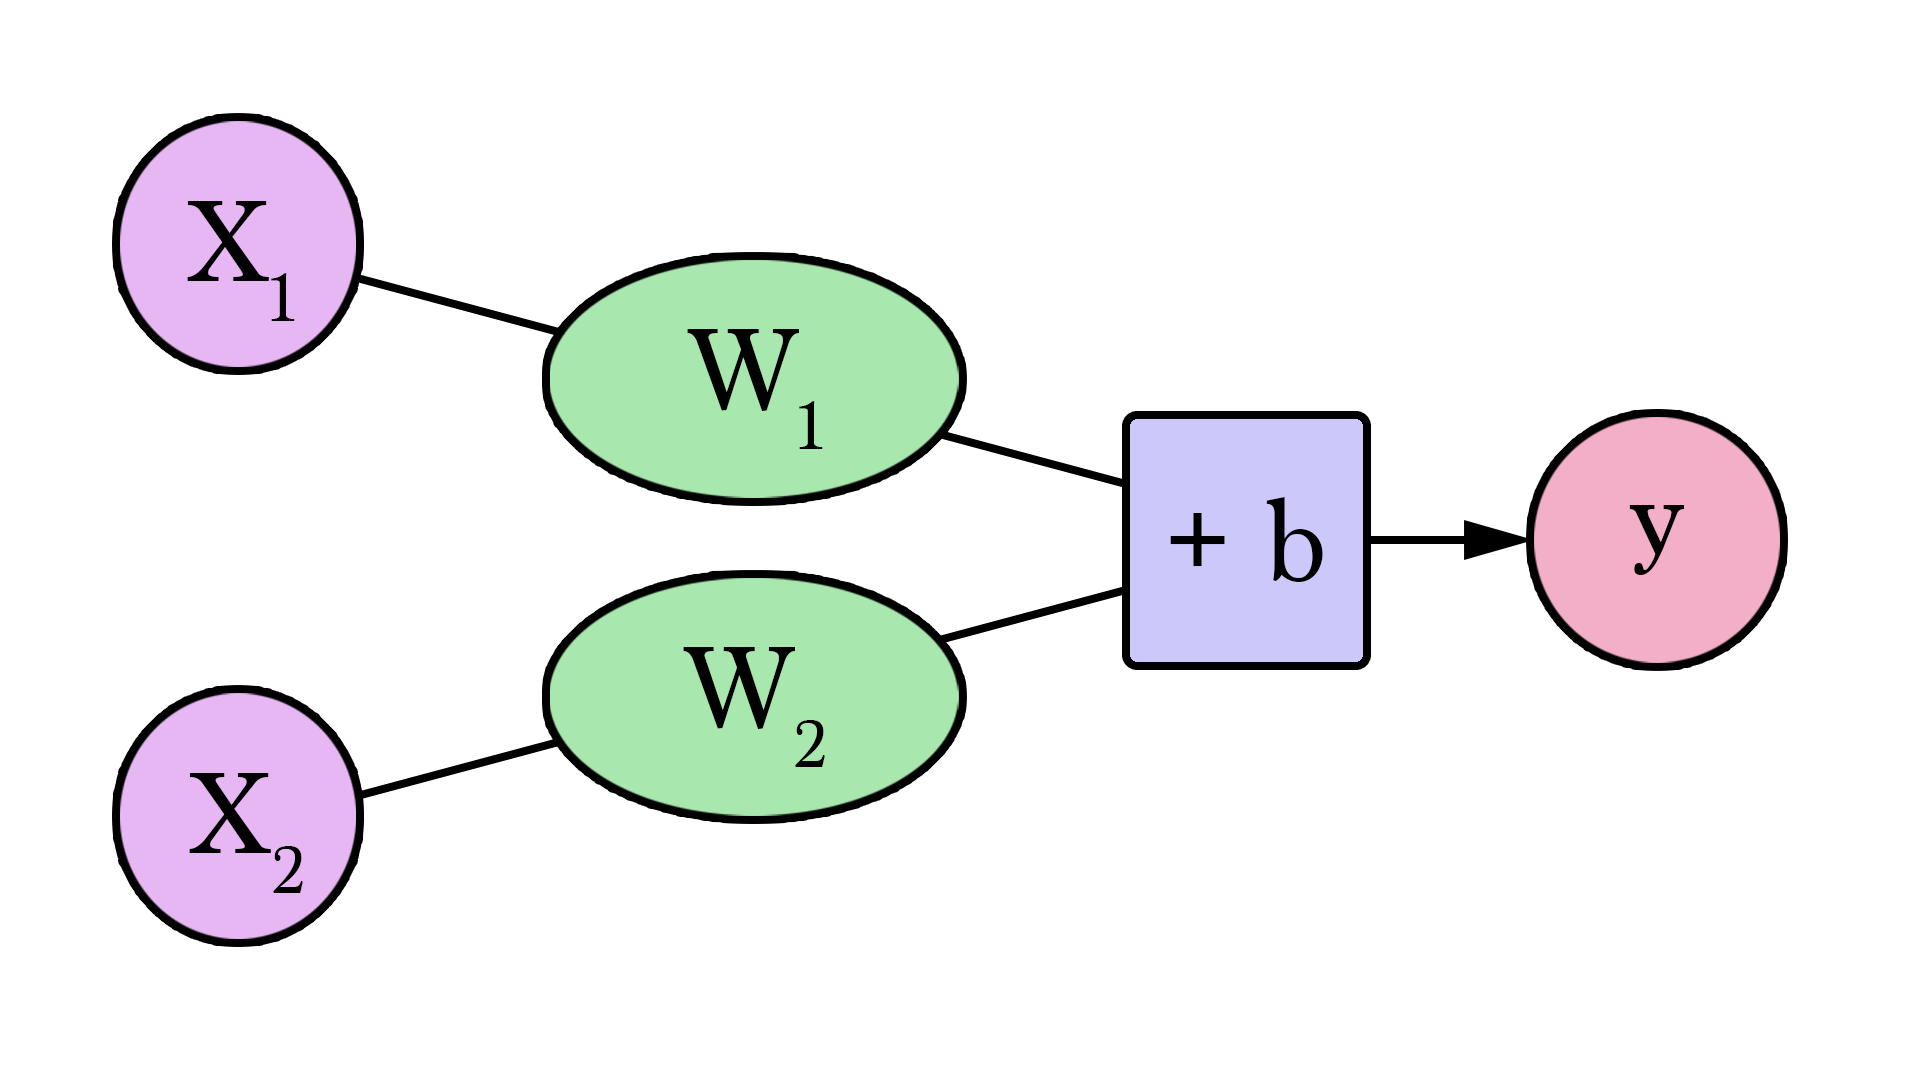
\includegraphics[width=.8\linewidth]{fig/NNs_2_variables.png}}
	\subfigure[Formula for the output of neuron on (a)]{\label{fig:basic_nn_b}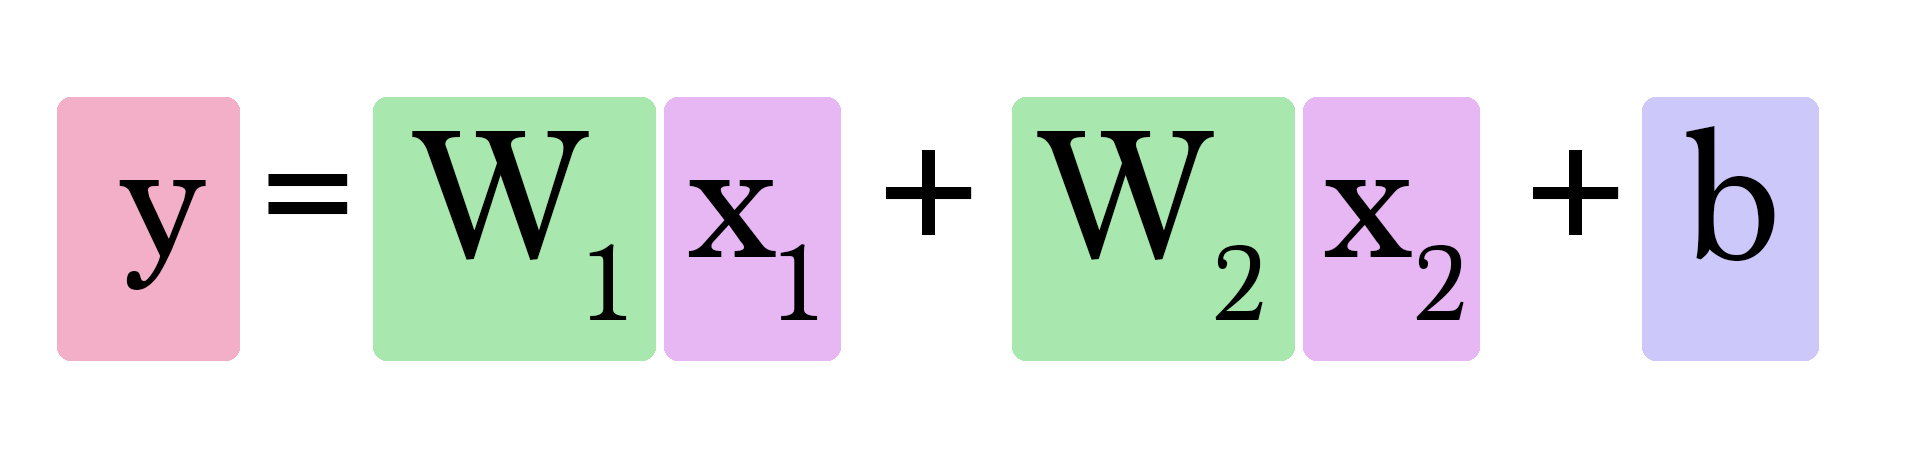
\includegraphics[width=.8\linewidth]{fig/NNs_formula_two_variables.png}}
	\vspace*{1mm}
	\captionfootnotemark{Sample Neuron.}
	\label{basic_neuron}
\end{figure}
\footnotetext{Retrieved from GitHub: \hyperrefurl{https://jalammar.github.io/visual-interactive-guide-basics-neural-networks/} on March 28, 2021.}

\section{The Basics of Deep Learning}

Let us take a look at basic deep learning terminologies. 

\begin{itemize}
	
	\item \textbf{Neural Network}: A neural network is a learning framework for machines using a collection of functions to understand and translate a data input into a desired output. The main inspiration is the human brain structure.
	
	\item \textbf{Nodes (Neurons)}: Neural networks are made of nodes (neurons). A node is a set of weights for that node and its associated nodes. Each node has an input data, a weight and a bias value.
	
	\item \textbf{Weight and Bias}: Weight transforms input data to the hidden layers of neural network. Some sources includes the bias into the weight. Both of them are learnable parameters, but bias is used and optimized to tune the distance between the predicted value and the intended value.
	
	\item \textbf{Batch}: A batch of data is a group selected from the whole data. The number of data in a batch are mostly chosen as a power of 2, such as $2^4, 2^5, 2^6$ etc \dots
	
	\item \textbf{Epoch}: An epoch is an iteration to learn through all train data. If batches are used, it is recommended to shuffle data order in each epoch before creating new batches on train data.
	
	\item \textbf{Train Data and Training}: The data group reserved to be used in learning process is called as train data. The ratio of the number of train data is generally determined as 80\% or 70\%, and the rest is placed into test data group. The train data must be strictly separated from validation and test data, and only used on training process. Training process is consisting of multiple epochs. In each epoch, the train data go into the model as input, the neural network works on learning from data, the losses and accuracy (if desired) are computed and the losses are optimized. If batching is used, this process is applied on each batch, and the average and final losses and accuracy (if desired) are calculated over all batches at the end of each epoch.
	
	\item \textbf{Validation Data and Validating}: If there exists enough train data for the problem and learning process, one may need to have validation data to validate the learning process periodically. The validation data group is strictly separated from train data such that generally the 80\% or 70\% of number of train data. During the validation process, the weights and biases are stable and no optimization process is applied, that is only the losses and other desired metrics, such as accuracy, are computed.
	
	\item \textbf{Test Data and Testing}: The data group reserved to be used in testing process is called as test data. The ratio of the number of test data is generally determined as 20\% or 30\%. The test data must be strictly separated from train data, and only used on testing process. The training process should not see any of test data. Testing process is usually only applied on the end of all epochs. However, when the train data is not feasible to be divided into validation data, at the end of each epoch testing process may be applied on test data. This method is also used to determine the overfitting and stop point.
	
	\item \textbf{Underfitting and Overfitting}: A learning algorithm is appeared to have underfitting when it cannot capture or fit the data well. On the other hand, when the model fits on the train data perfectly, it may be started actually to memorize the train data, not learn from the data. Therefor, the testing metrics are seen in the opposite direction of what is desired. This situation is called as overfitting.
	
	\begin{figure}[h]
		\centering
		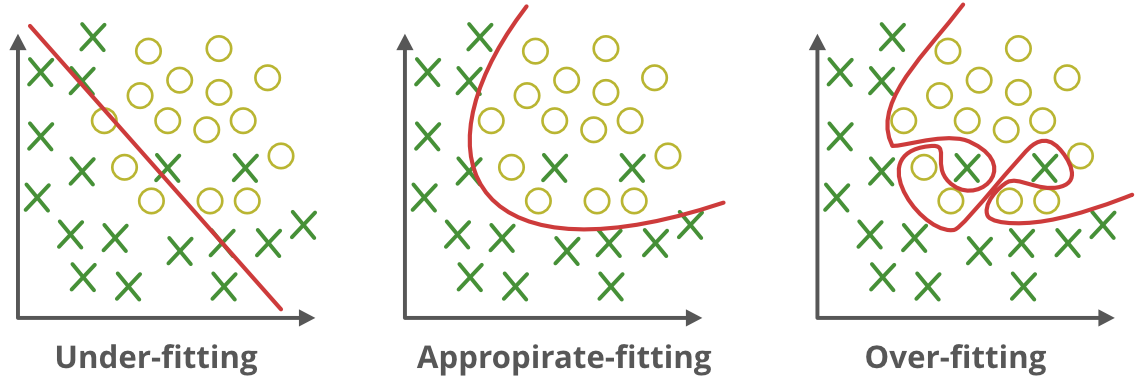
\includegraphics[width=.8\linewidth]{fig/underfitting_overfitting.png}
		\vspace*{1mm}
		\captionfootnotemark{Underfitting - Well Fitting - Overfitting.}
		\label{underfitting_overfitting}
	\end{figure}
	\footnotetext{Retrieved from GeeksforGeeks: \hyperrefurl{https://www.geeksforgeeks.org/underfitting-and-overfitting-in-machine-learning/} on March 28, 2021.}
	
\end{itemize}

\section{The Cross-Entropy Loss Function}\label{sec:CH3_cross_entropy}

The loss function is the function that represents the error between predicted and true values, which can be called as the cost, of the problem to be optimized.

The cross-entropy loss function is one of the most used loss functions to measure the performance of corresponding classifier. The function maps the probability values between 0 and 1 to the cost value. Here the loss value increases together with the divergence between the true label and the predicted probability.

The cross-entropy loss function is as in the equation (\ref{eq:cross_entropy_loss_formulae}).

\begin{equation}
	\label{eq:cross_entropy_loss_formulae}
	L_{cross-entropy} = - \sum_{i=1}^{n} y_{i} \log(p_{i}) \:,
\end{equation}

where $n$ is the number of classes, and $y_{i}$ and $p_{i}$ are the truth label and Softmax probability respectively for the $i^{th}$ class. Thus, for a binary classification problem, the cross-entropy loss function can be taken as in the equation (\ref{eq:binary_cross_entropy_loss_formulae}).

\begin{equation}
	\label{eq:binary_cross_entropy_loss_formulae}
	L = - \left ( y\:\log(p) + (1 - y)\:\log(1-p) \right ) \:,
\end{equation}

where $y$ and $p$ are the binary indicator (0 or 1) depends on the correctness of observed class label and the probability of observation respectively.

\section{The Basics of Optimization Methods}
\label{sec:CH3_the_basics_of_optimization}

To reduce the losses and to reach the more accurate possible predictions, various optimization methods can be used. The weights are initialized and updated on each training epoch. The initialization strategies may vary depending on the neural network. It is aim to achieve the most satisfying results by using some algorithms called as optimizers.

\subsection{Stochastic Gradient Descent with Momentum (SGD) Optimization Algorithm}

Stochastic gradient descent is an iterative method for optimizing an objective function with suitable smoothness properties. It can be regarded as a stochastic approximation of gradient descent optimization. Momentum remembers the weight update at each iteration, and determines the next update as a linear combination of the gradient and the previous update \cite{SGD_Momentum}.

\begin{figure}[h]
	\centering
	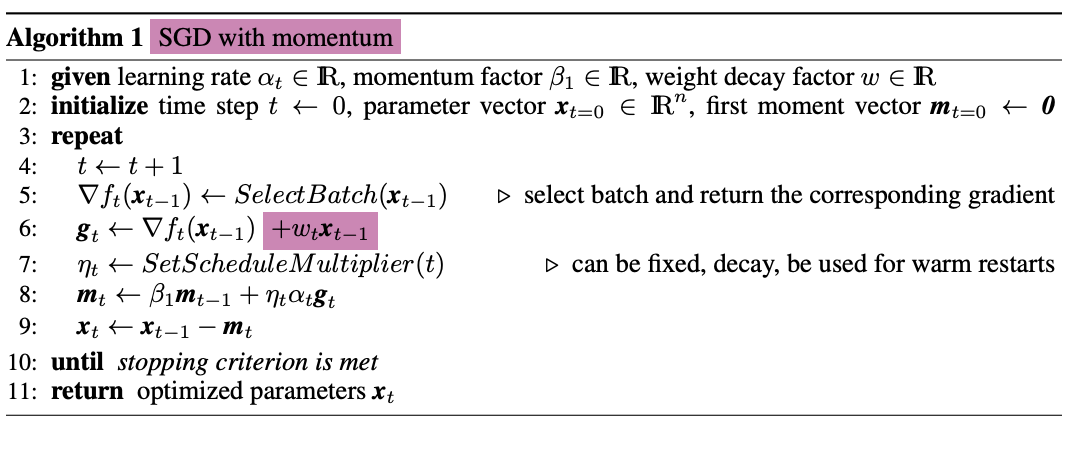
\includegraphics[width=\linewidth]{fig/sgd_momentum.png}
	\caption{Pseudocode for SGD with Momentum \cite{weight_decay_regularization}.}
	\label{sgd_momentum}
\end{figure}

\subsection{Adam Optimization Algorithm}

Adaptive moment estimation is an optimization algorithm that uses the running averages of both the gradients and the second moments of the gradients. Before each step, the gradient of loss function is calculated and a step in the opposite direction is taken with corresponding rate. This process is also called as Adam with L2 regularization \cite{Adam}.

\subsection{Adam with Decoupled Decay (AdamW) Optimization Algorithm}

Adam with decoupled weight decay does not use the regularization as the normalized by square root of second moment vector. Thus, it is only proportional to the weight itself \cite{Adam}.

\begin{figure}[h]
	\centering
	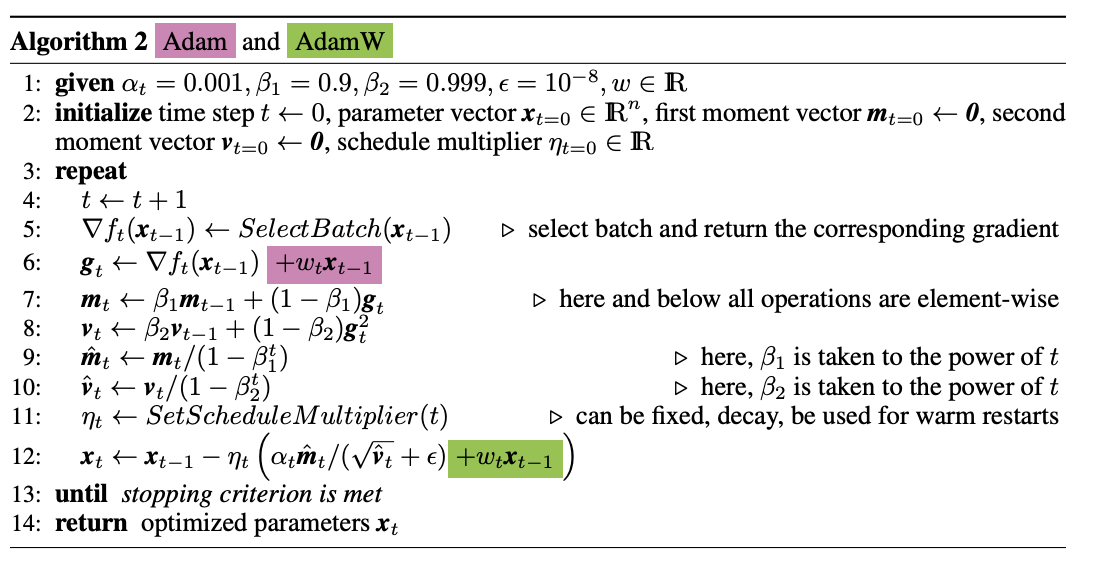
\includegraphics[width=\linewidth]{fig/adam_n_adamw.png}
	\vspace*{1mm}
	\caption{Pseudocode for Adam and AdamW \cite{weight_decay_regularization}.}
	\label{adam_and_adamw}
\end{figure}

\section{The Basics of Convolutional Neural Networks} \label{basics_of_cnn}

The convolutional neural networks (CNNs) are the special study and research area of deep neural networks. They are mostly used in visual problem analyzing and solving.

Basically, a CNN model consists of three parts such that an input layer, hidden layers and an output layers. The structure of CNNs comports with the feed-forward networks. That is, the information only goes through in one direction, forward. To feed and train a feed-forward network, backpropagation algorithm is commonly used. The algorithm orders to compute the gradients in weight space of a feed-forward network, with respect to a loss function. Then the weight space is updated with these gradients by the method of corresponding optimizer. The gradient of objective loss function $ f(\textbf{$\theta$}) $ at a weight vector \textbf{$\theta_{t}$} is computed via directional derivatives and chain rule, and represented by $ \nabla f(\textbf{$\theta_{t}$}) $. 

An example of using directional derivatives and chain rule can be found in Figure~\ref{fig:compute_gradient}. Assume there exist $m$ number of $x_{i}$ nodes feeding $y$ where $\textbf{x} = (x_{1}, \dots , x_{m})$ is m-dimensional vector. Then the gradient of $y$ at $\textbf{x}$ is constructed as $\nabla y (\textbf{x}) = {\begin{bmatrix}{\frac {\partial y}{\partial x_{1}}}(\textbf{x})\\\vdots \\{\frac {\partial y}{\partial x_{m}}}(\textbf{x})\end{bmatrix}}$.

\begin{figure}[h]
	\centering
	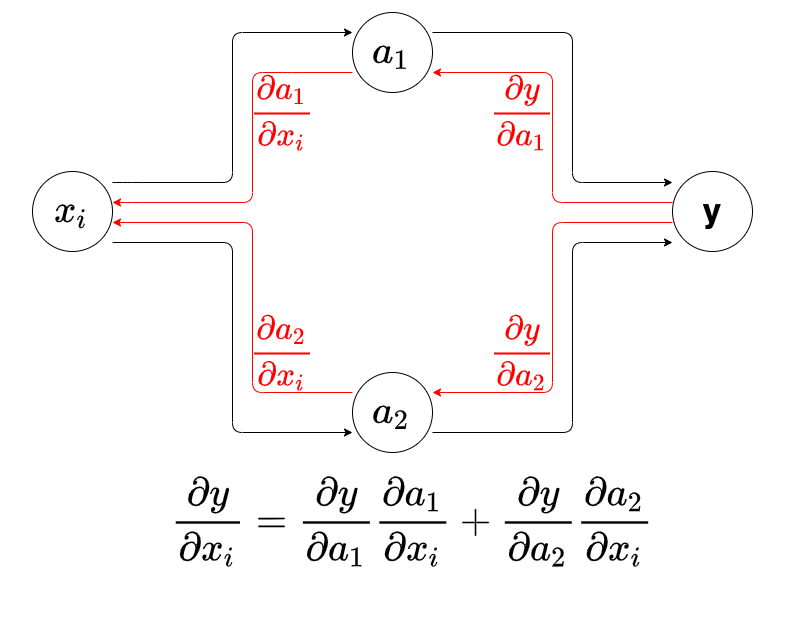
\includegraphics[width=.6\linewidth]{fig/gradient_example.png}
	\vspace*{1mm}
	\caption{The usage example of directional derivatives and chain rule.}
	\label{fig:compute_gradient}
\end{figure}

In this section and its subsections we study on the fundamental layers and elements of CNN architectures. 

\begin{figure}[h]
	\centering
	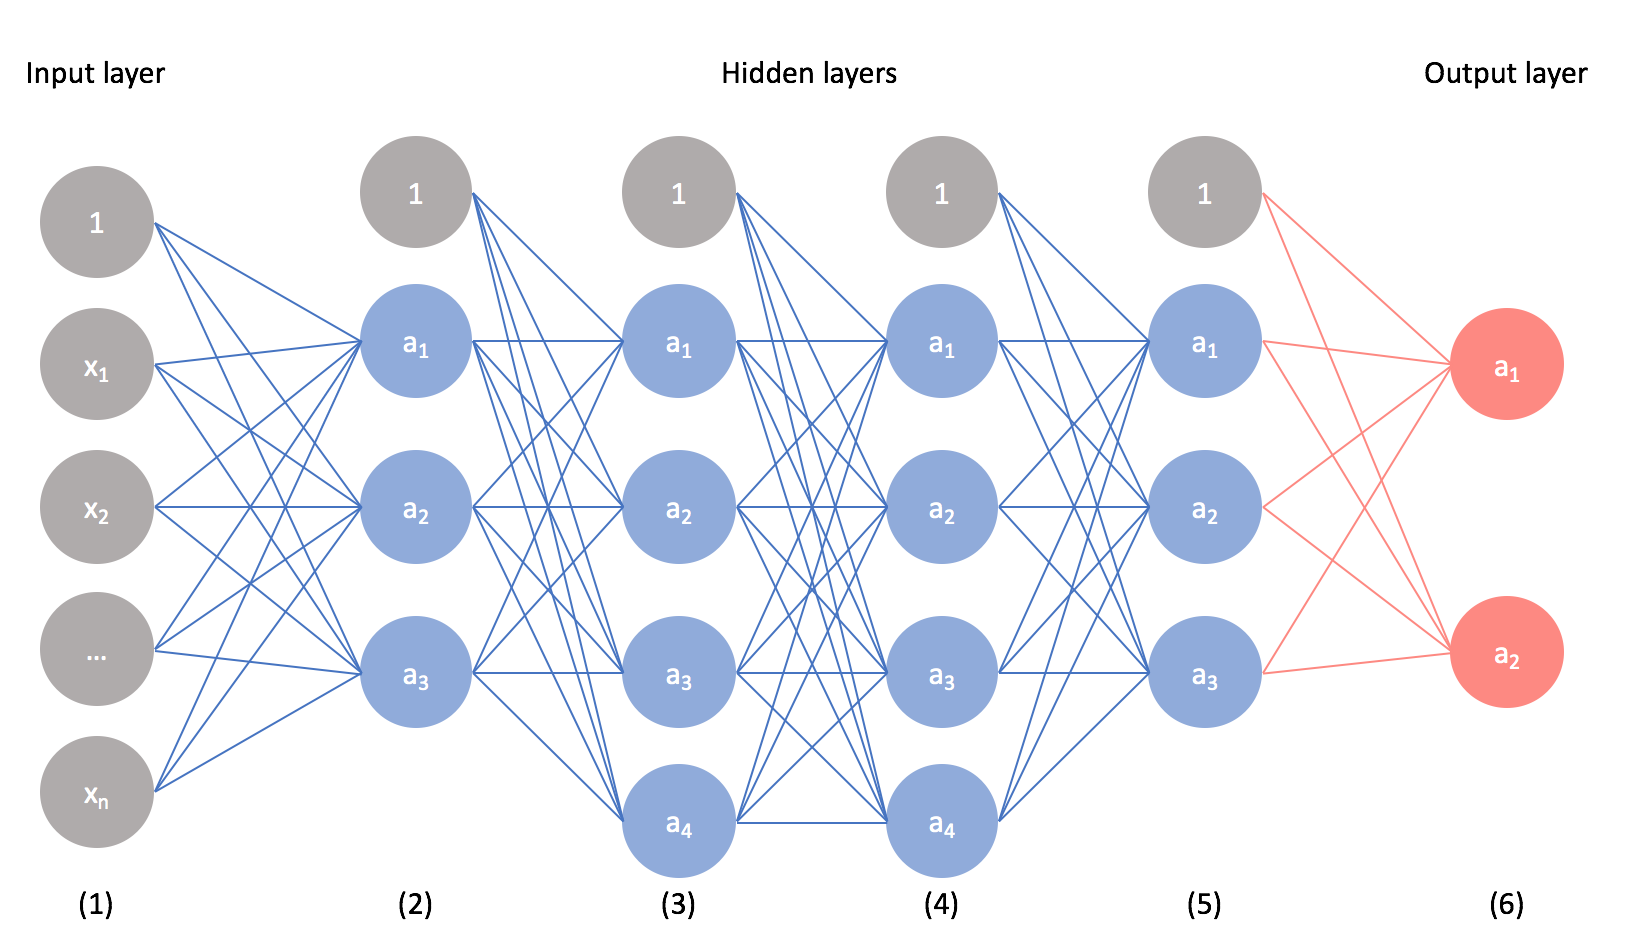
\includegraphics[width=.8\linewidth]{fig/basic_cnn_sample.png}
	\vspace*{1mm}
	\captionfootnotemark{Sample CNN Architecture.}
	\label{basic_cnn_sample}
\end{figure}
\footnotetext{Retrieved from: \hyperrefurl{https://www.jeremyjordan.me/convolutional-neural-networks/} on March 31, 2021.}

\subsection{Convolutional Layer}

Convolutional layer is the building block of CNN architectures and is used to reveal the distinctive features of input data. The various filters are applied to the data to reveal low and high-level feature map. After convolution, the size of the input data changes depending on the filter (or kernel), stride and padding choices. The outputs of the convolution layers are called activation maps.

A convolution layer includes a window named as filter or kernel that can be of different sizes as $2x2$, $3x3$, etc.. The coefficients that filters include change on each iteration during the training of a CNN. This coefficients and their updates are used to detect the significant and learnable parts of the data.

Filter is started to be applied from the upper left corner, and continues moving towards the right. When there are no cells left to be scanned on the right, it continues from the lower cells as before. On each step, the filter and the corresponding area of input matrix are multiplied by element-wise. The step length of scanning process is called as stride. The default stride value is 1; however, different stride values may be used depends on the data and CNN architecture. If the stride is set as $s$, then the kernel window move by jumping $s$ cells.

On some situations, such as a size inconsistency or paying attention to the information on the edges and corners of the image, the edges of input matrix may be filled by zeros. These process is calling as padding. If the padding value is set as $p$, the $p$ cells with zero values are added to the edges of input matrix.

\begin{figure}[h]
	\centering
	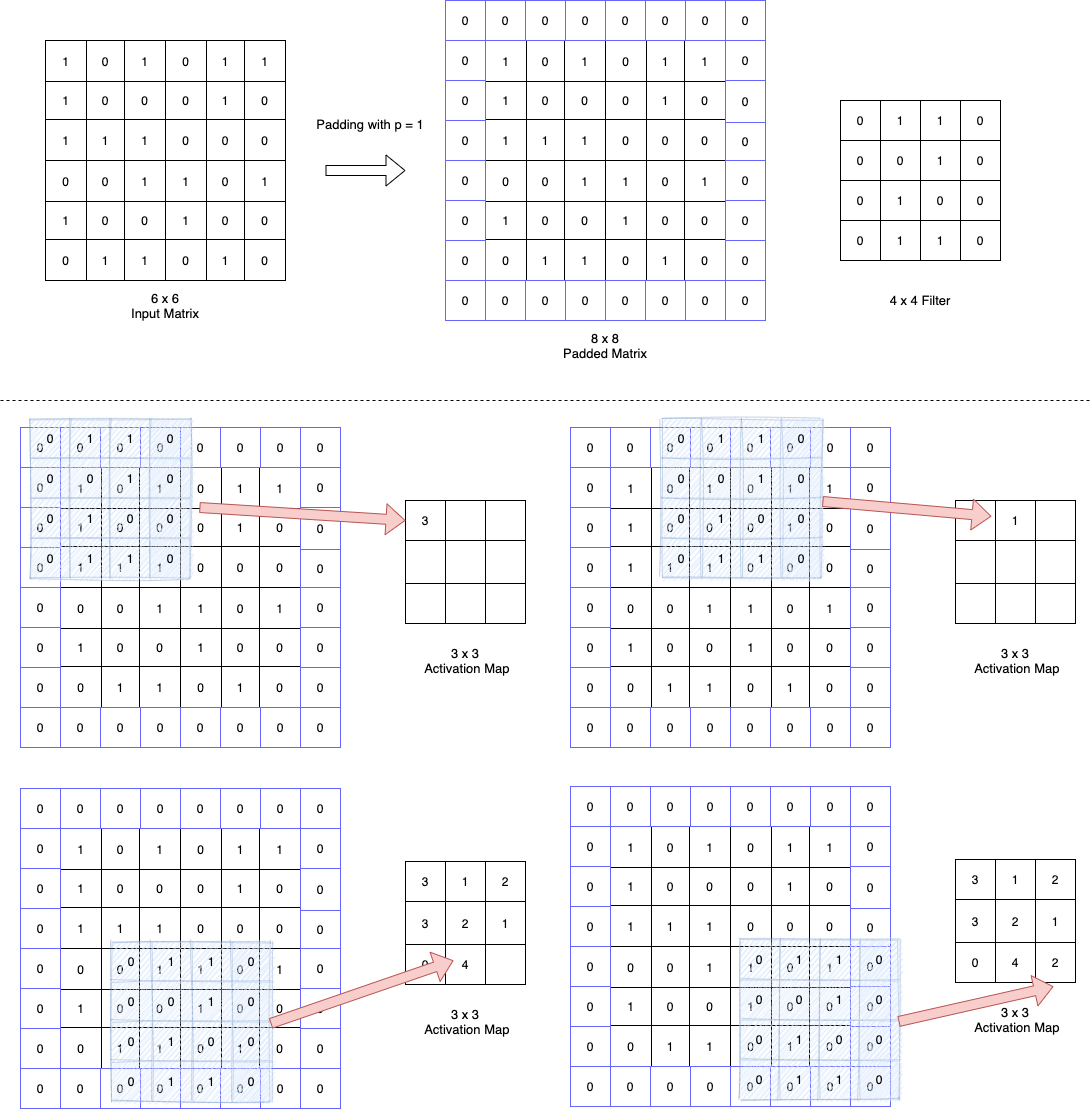
\includegraphics[width=\linewidth]{fig/conv_layer.png}
	\vspace*{2mm}
	\caption{Activation map construction by 4 x 4 filter window with stride as 2.}
	\label{conv_layer}
\end{figure}

The Figure~\ref{conv_layer} gives a summary about how activation map is constructed for a given input matrix and a filter. Let us give a detailed example to about it. Assume that the input data is a three layered, which are red, green and blue, image in the shape of 223 x 223 x 3, and the padding size is 1. Let choose two filter windows in the size of 5 x 5 and the step size (stride) as 2. Let denote the input size with $W_{input} x H_{input} x D_{input}$, the padding with $P$, the number of filters with $K$, the size of a filter window with $F x F$ and the stride with $S$. Here, we have:

\begin{itemize}
	\item $W_{input} = 223, \: H_{input} = 223, \: D_{input} = 3$,
	\item $K = 2, \: F = 5$,
	\item $P = 1, \: \text{and} \: S = 2$.
\end{itemize}

The size of activation map is calculated as:

\begin{flalign}
	\label{activation_map_w_output}
	&W_{output} = (W_{input} - F + 2P)\,/\,S + 1\:, \\
	\label{activation_map_h_output}
	&H_{output} = (H_{input} - F + 2P)\,/\,S + 1\:,\quad\text{and} \\
	\label{activation_map_d_output}
	&D_{output} = K\:.
\end{flalign}

Consequently, the activation map is yielded in the size of 112 x 112 x 2 by the equations  (~\ref{activation_map_w_output}), (~\ref{activation_map_h_output}) and (~\ref{activation_map_d_output}) respectively. 

\subsection{Activation Function (Rectified Linear Units - ReLU)}

The activation function forms the output of the node for a given input or input set. Rectifier activation function maps the input to non-negative values. A unit form of the rectifier activation function, which is given in equation (\ref{eq:relu_formula}), is called as Rectified Linear Units (ReLU) which is the most common used in neural networks.

\begin{equation}
	\label{eq:relu_formula}
	\text{ReLU is defined as:}\quad
	f(x) = \max(0, x) \:.
\end{equation}

\subsection{Pooling Layer}

Pooling layers are commonly used in between the convolutional layers, especially after activation functions. A pooling layer outputs a a new feature map with the lower size than the size of input feature map. The characteristics of output feature map is depends on the type of pooling layer. The pooling layers have a stride parameter to control the step size of the movement of pooling window. The most common pooling functions are given below.

\begin{itemize}
	\item \textbf{Average Pooling:}  The average of corresponding window is computed and inserted into output feature map.
	\item \textbf{Maximum Pooling:}  The maximum value of corresponding window is inserted into output feature map.
\end{itemize}

\begin{figure}[h]
	\centering
	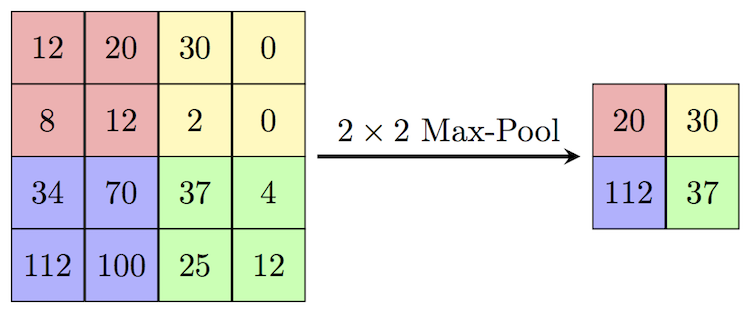
\includegraphics[width=.8\linewidth]{fig/MaxpoolSample.png}
	\captionfootnotemark{Maximum pooling operation sample with 2 x 2 window and stride as 2.}
	\label{fig:maxpooling}
\end{figure}
\footnotetext{Retrieved from: \hyperrefurl{https://computersciencewiki.org/index.php/Max-pooling_/_Pooling} on April 3, 2021.}

\subsection{Batch Normalization}

Batch normalization is a technique for training the deep neural networks that standardize the inputs to one layer for each mini batch. This has the effect of stabilizing the learning process and significantly reducing the number of training epochs required \cite{A_novelCNNModel}.

\subsection{Dropout}

Dropout is the removing operation of the nodes below certain threshold value in the network at each training iteration. In other words, it is aimed not to use weak information and memorize the network. Dropout can be in any layer and its threshold value, which can differ in different layers,  is between [0,1].

\begin{figure}[h]
	\centering
	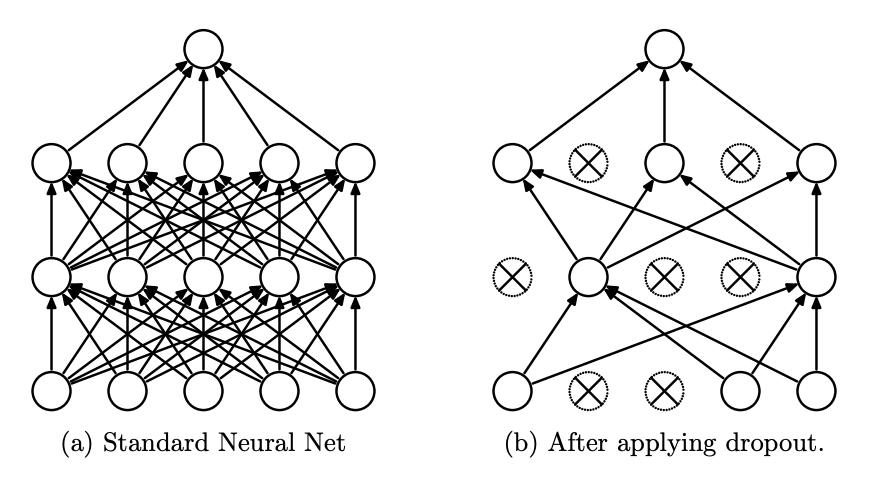
\includegraphics[width=.8\linewidth]{fig/dropout.png}
	\caption{(a) A standard neural network, (b) A neural network after applying dropout\cite{dropout_article}.}
	\label{fig:dropout}
\end{figure}

\subsection{Flattening}

Flatten operation reshapes the input into the one-dimension. It is used before passing to the fully-connected layers.

\subsection{Fully-Connected Layer}

This structure is used to combine the information in the previous layers. It pre requires the flatten operation before itself. The fully-connected layers are used to classify data in different categories, or construct feature maps to be used in another artificial network methods.

\begin{figure}[h]
	\centering
	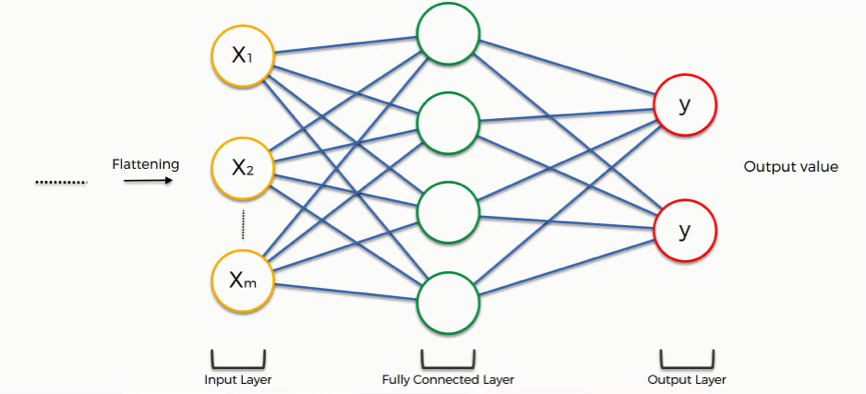
\includegraphics[width=\linewidth]{fig/fully_connected_layer.png}
	\vspace*{1mm}
	\captionfootnotemark{The usage of full-connected layer for a binary classifier.}
	\label{fig:fully_connected_layer}
\end{figure}
\footnotetext{Retrieved from: \hyperrefurl{https://www.superdatascience.com/blogs/convolutional-neural-networks-cnn-step-4-full-connection} on April 3, 2021.}

\section{Transfer Learning}

Transfer learning is transferring the features, weights, etc. in pre-trained model to another artificial learning model. This can be between two deep learning models or across a machine learning and deep learning model. In this thesis, the weight transfer from pre-trained CNN models to CNN models and feature transfer from CNN models to machine learning models are used.

Transfer earning is used to shorten the training time if the data set is insufficient and to achieve high performance with less data. If the data on each class is less than 1000, the dataset may be considered as small. 

To prepare a pre-trained CNN model for visual artificial intelligence problems, ILSVRC 2012 ImageNet \cite{imagenet} dataset, including 1000 class with large data, is commonly used. The weights after the training process is saved and shared to use in transfer learning afterwards. On transfer learning, the pre-trained model is called with its pre-computed weights, and the weights are transferred into the same empty neural network. There exist different approaches to train this new neural network; such that, training the all layers on the convolutional block, training a part of the layers on the convolutional block and freezing the other, or freezing all layers on the convolutional block. The choice of strategy, which is called as fine-tuning operation, depends on the size of dataset and the similarity between the dataset used in pre-training process and the dataset to be used in current task. Then the last fully-connected layer is adapted to the current task by updating itself or adding new fully-connected layers.

\begin{figure}[h]
	\centering
	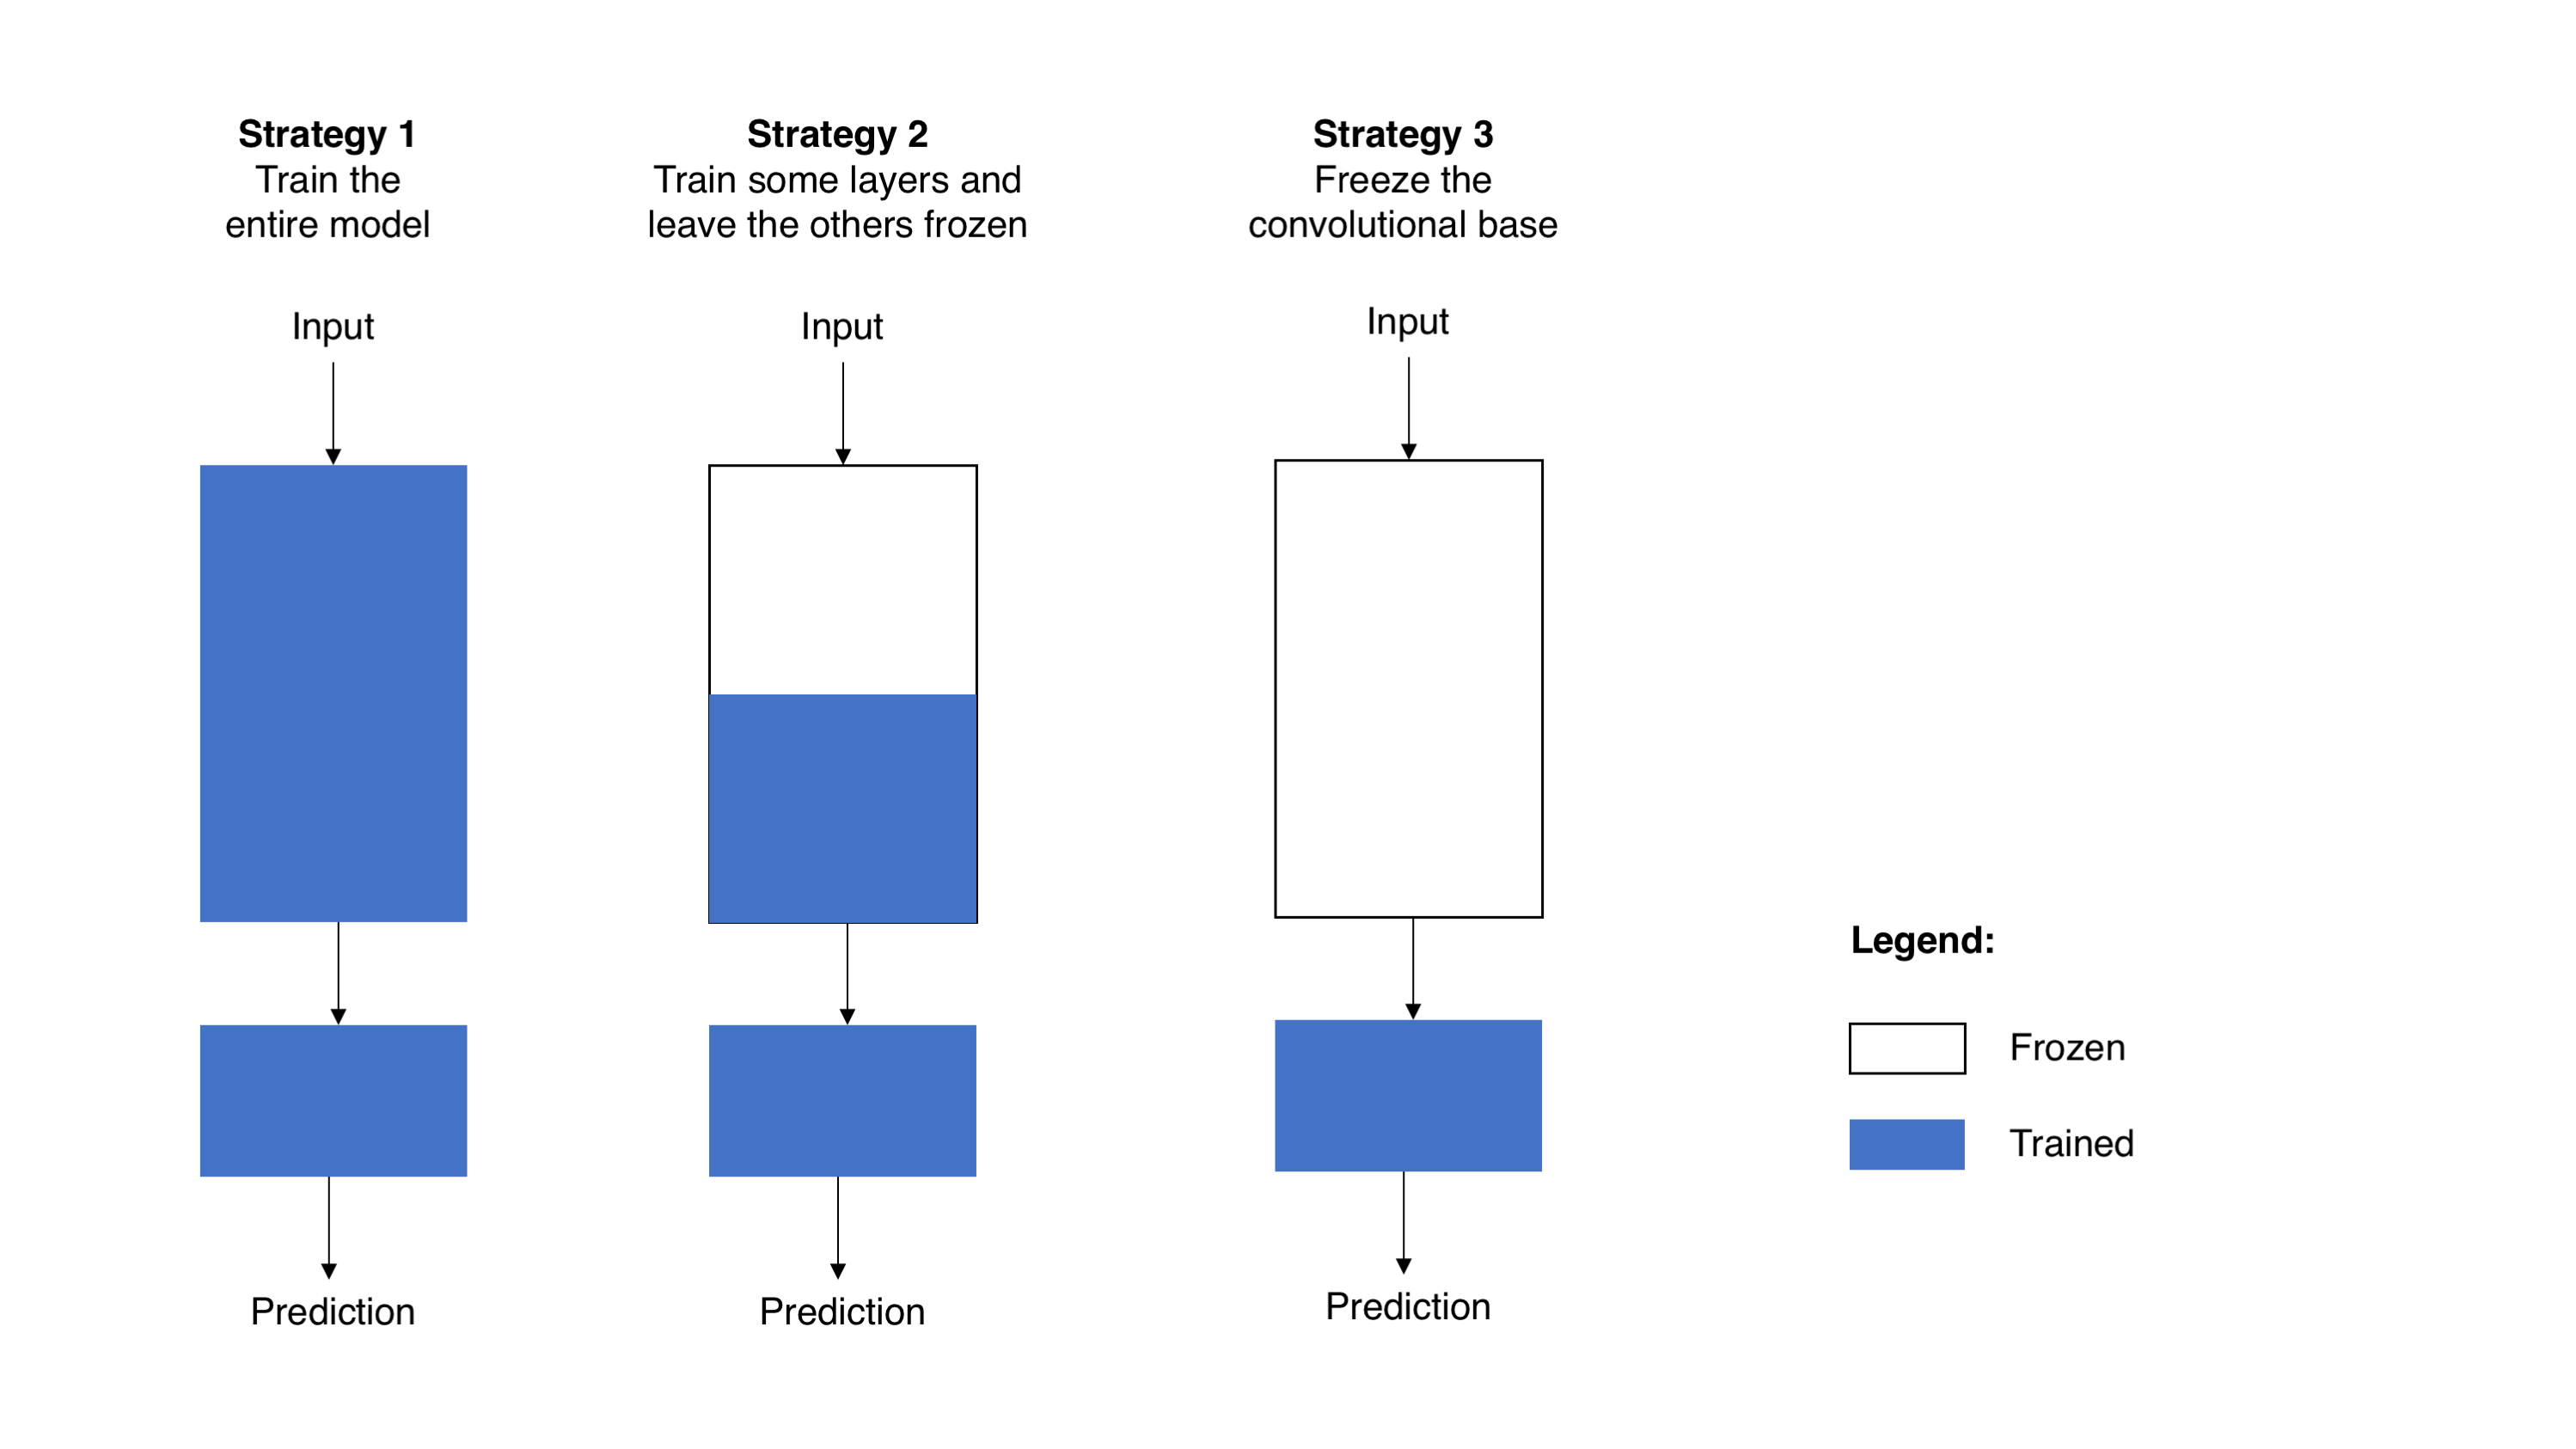
\includegraphics[width=.8\linewidth]{fig/pretrain_strategies.png}
	\vspace*{1mm}
	\captionfootnotemark{Different fine-tuning strategies on pre-trained model.}
	\label{fig:pretrain_strategies}
\end{figure}
\footnotetext{Retrieved from: \hyperrefurl{https://towardsdatascience.com/transfer-learning-from-pre-trained-models-f2393f124751} on April 3, 2021.}

To prepare a deep feature set to be used in another artificial learning model, such as machine learning models, the features on a fully-connected layer, mostly the first or second, are extracted and saved. Then the saved deep features are used in the target artificial learning model as the feature map of dataset.

\begin{figure}[h]
	\centering
	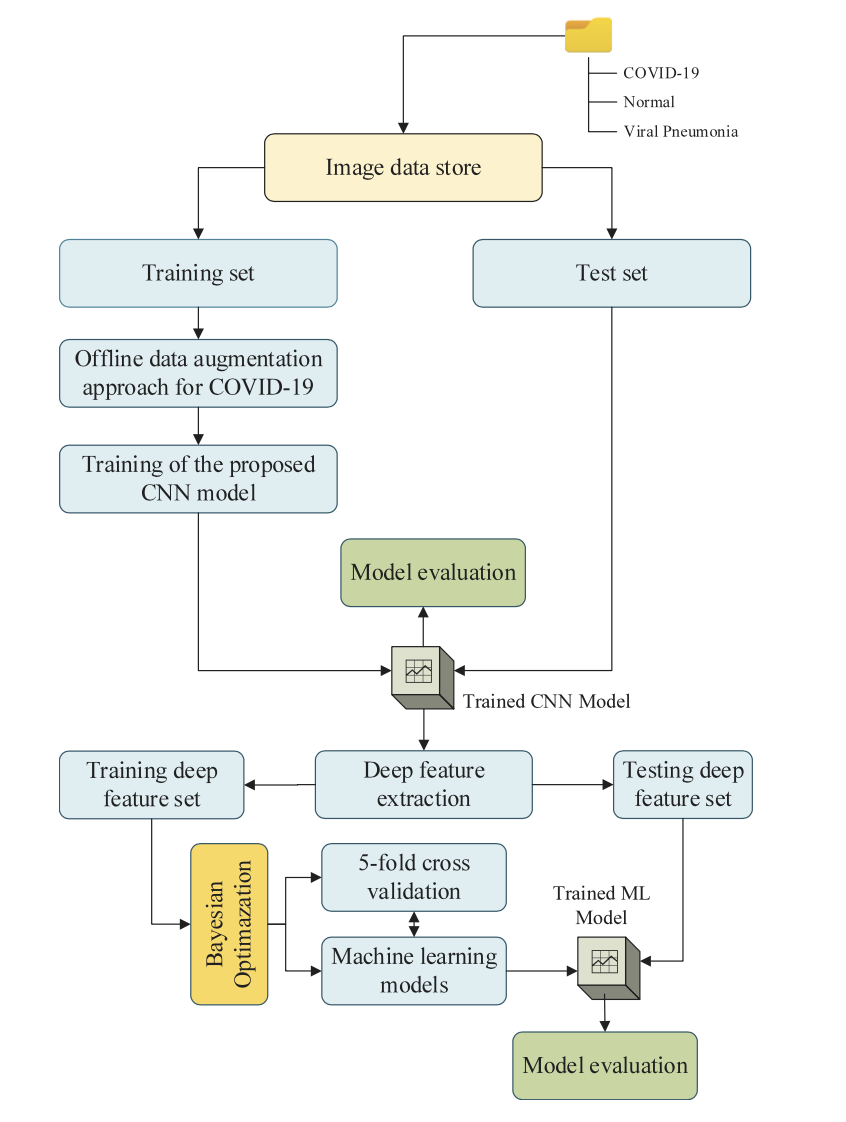
\includegraphics[width=.8\linewidth]{fig/deepfeauter_usage.png}
	\caption{Deep feature extraction from CNN models and using them in machine learning models \cite{A_novelCNNModel}.}
	\label{fig:A_novelCNNModel_architecture}
\end{figure}

\section{CNN Models}

There are too many similar and different CNN architectures which can be simply called as models. These models consist of various combinations of input layer, hidden layers and an output layer such that some basics of them are explained in Section~\ref{basics_of_cnn}.

In this section, the state-of-the-art CNN models used in the thesis are introduced and detailed.

\subsection{AlexNet}

The AlexNet architecture was developed by Krizhevsky et al. \cite{AlexNet} for the object recognition problem. This model was trained with the ILSVRC 2012 ImageNet \cite{imagenet} dataset, and achieved high performance results and won first place in the ImageNet competition in 2012. There are 8 layers in total in the AlexNet architecture. The first five are convolution, which uses 11x11 size filters with the stride as 4, and some are supported by the maximum pooling layer, the remaining three are the fully-connected layers. The ReLU activation function is used after each convolution and fully-connected layer. The size of the input image is 224 × 224 × 3, and the number of filters used increases as going deeper into the model.

\begin{figure}[h]
	\centering
	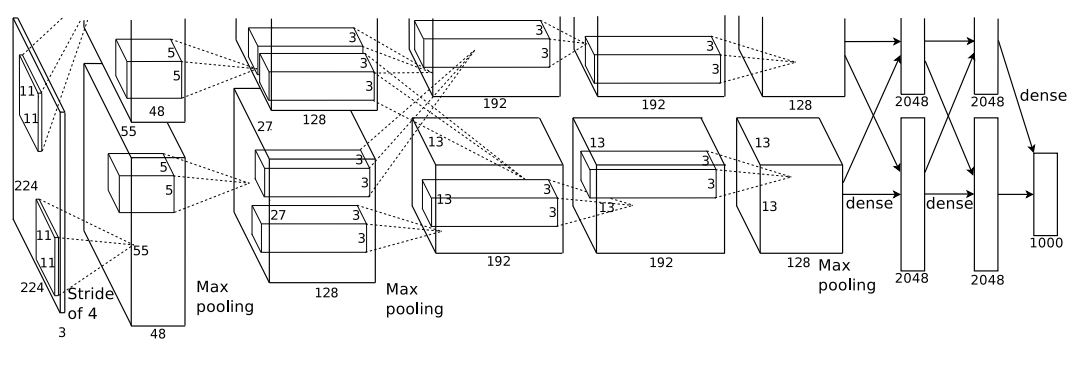
\includegraphics[width=\linewidth]{fig/alexnet_arch.png}
	\caption{An illustration of AlexNet architecture with input image in the size of 224 × 224 × 3 \cite{AlexNet}.}
	\label{fig:alexnet_arch}
\end{figure}

\subsection{Residual Neural Network (ResNet)}

The residual neural network architectures was announced by He et al. \cite{ResNet} to avoid the vanishing and exploding gradient problems by using residual blocks. A residual block is simply a connection which allows to take the activation from one layer and feed it to another layer in much deeper. This model achieved high performance results on ILSVRC 2015 ImageNet \cite{imagenet} dataset, and won the 1st place on the corresponding task.

\begin{figure}[h]
	\centering
	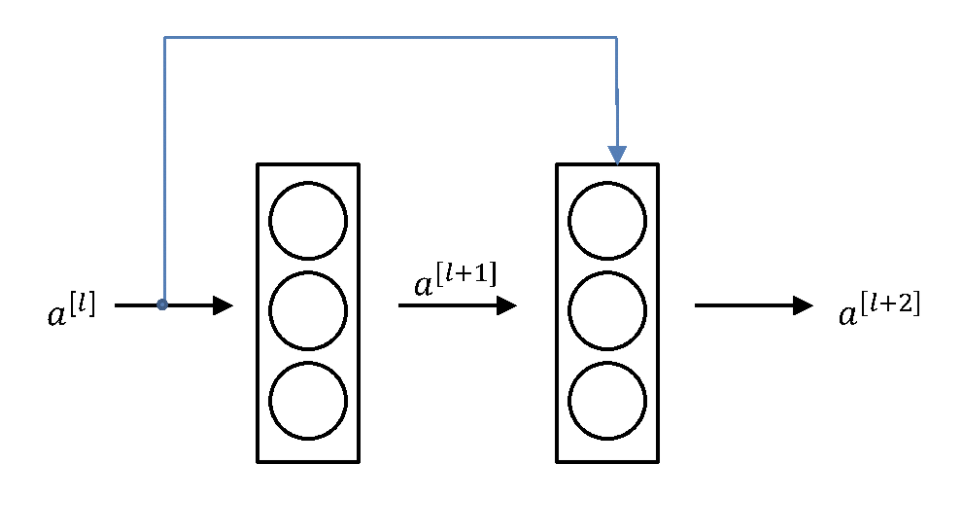
\includegraphics[width=.6\linewidth]{fig/residual_block.png}
	\captionfootnotemark{An illustration for residual block. Here, $a^{[l]}$ is the starting activation layer and $a^{[l+2]}$ is the fed activation layer.}
	\label{fig:residual_block}
\end{figure}
\footnotetext{Retrieved from: \hyperrefurl{http://datahacker.rs/deep-learning-residual-networks/} on April 4, 2021.}

\begin{figure}[h]
	\centering
	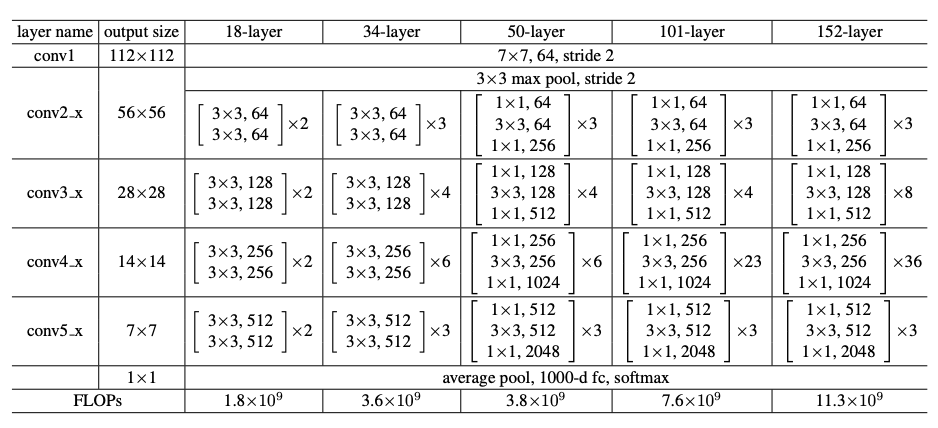
\includegraphics[width=\linewidth]{fig/resnet_archs.png}
	\vspace*{1mm}
	\caption{The ResNet architectures\cite{ResNet}.}
	\label{fig:resnet_archs}
\end{figure}

\subsubsection*{\textit{ResNet-18}}

The first convolution layer includes a 7 x 7 filter and scans with stride as 2, then maximum pooling is applied with 2 x 2 window and stride as 2. Afterwards, 8 residual blocks, such that each of them includes 2 convolutional layers with 3 x 3 filters, come. That is, there exist 16 convolutional layers inside of residual blocks. After the residual blocks, there is an average pooling following with a fully-connected layer with 1000 neurons, which represents the class number.

\subsubsection*{\textit{ResNet-34}}

The first convolution layer includes a 7 x 7 filter and scans with stride as 2, then maximum pooling is applied with 2 x 2 window and stride as 2. Afterwards, 16 residual blocks, such that each of them includes 2 convolutional layers with 3 x 3 filters, come. That is, there exist 32 convolutional layers inside of residual blocks. After the residual blocks, there is an average pooling following with a fully-connected layer with 1000 neurons, which represents the class number.

\subsubsection*{\textit{ResNet-50}}

The first convolution layer includes a 7 x 7 filter and scans with stride as 2, then maximum pooling is applied with 2 x 2 window and stride as 2. Afterwards, 16 residual blocks, such that each of them includes 3 convolutional layers with 1 x 1, 3 x 3 and 1 x 1 filters in order, come. That is, there exist 48 convolutional layers inside of residual blocks. After the residual blocks, there is an average pooling following with a fully-connected layer with 1000 neurons, which represents the class number.

\subsection{VGG}

Simonyan and Zisserman \cite{VGG} proposed a very profound architecture for the problem of image recognition. It is aimed to achieve higher classification performance by using a small size filter and increasing the depth of the model. This model was trained with the ILSVRC 2012  ImageNet \cite{imagenet} dataset and achieved high success results. This study has proven the importance of depth in image description models.

\begin{figure}[h]
	\centering
	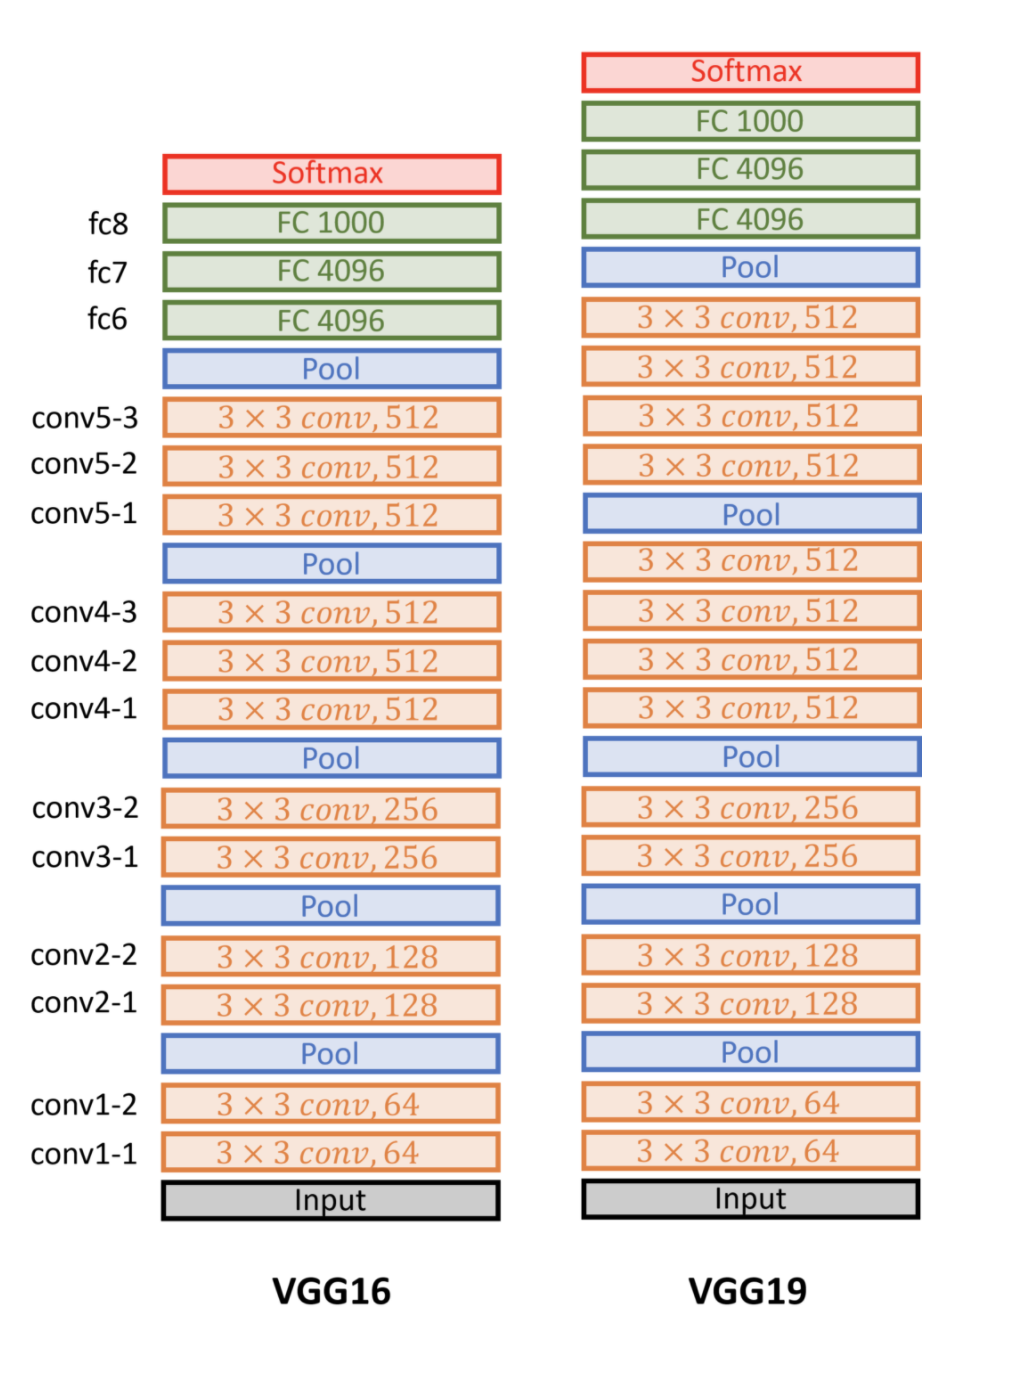
\includegraphics[width=.6\linewidth]{fig/vgg16_vgg19_archs.png}
	\captionfootnotemark{An illustration of VGG architectures.}
	\label{fig:vgg16_vgg19_archs}
\end{figure}
\footnotetext{Retrieved from: \hyperrefurl{http://datahacker.rs/deep-learning-vgg-16-vs-vgg-19/} on April 4, 2021.}

\subsubsection*{\textit{VGG16}}

The input layer of the model architecture starts with a 24 × 24 color image, and there are 12 convolution layers using 3 × 3 filters. There are a total of 5 maximum pooling layers used after some convolution layers. In maximum pooling, 2 x 2 windows were used with stride as 2. After the convolution layers, there are three fully-connected layers such that the first two of which are 4096 neurons and the last one is 1000 neurons, which represents the class number. The ReLU activation function was used after all the hidden layers.

\subsubsection*{\textit{VGG19}}

The input layer of the model architecture starts with a 24 × 24 color image, and there are 14 convolution layers using 3 × 3 filters. There are a total of 5 maximum pooling layers used after some convolution layers. In maximum pooling, 2 x 2 windows were used with stride as 2. After the convolution layers, there are three fully-connected layers such that the first two of which are 4096 neurons and the last one is 1000 neurons, which represents the class number. The ReLU activation function was used after all the hidden layers.